\begin{figure}
\centering
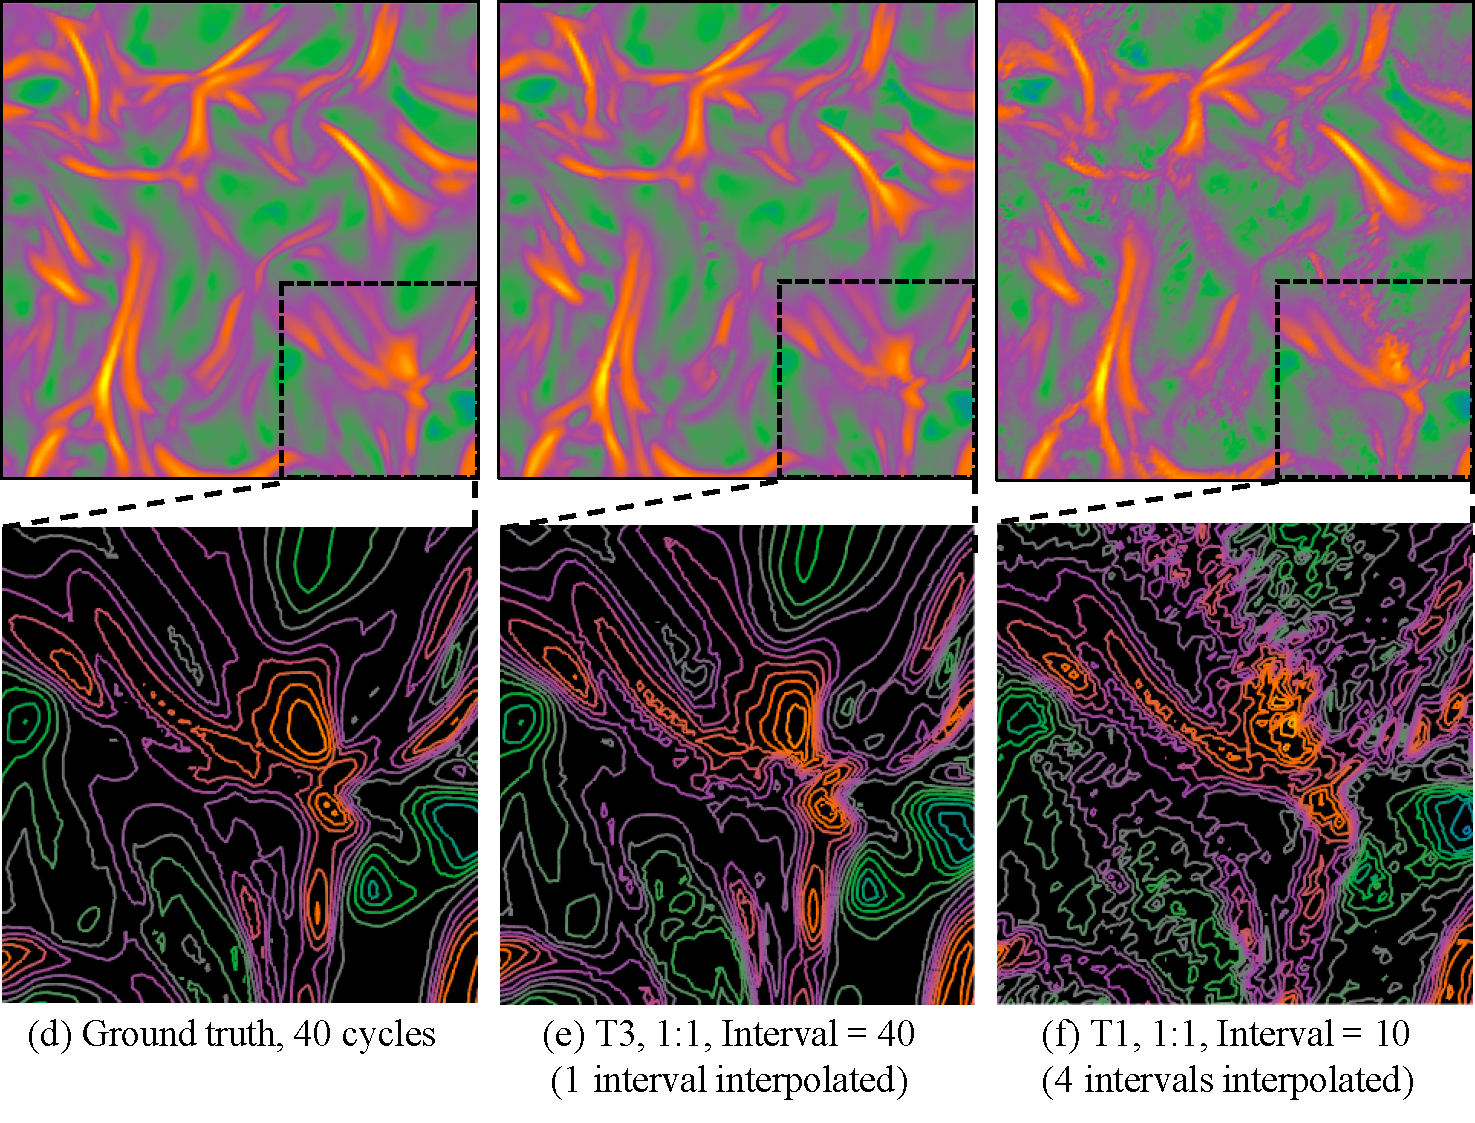
\includegraphics[width=\linewidth,keepaspectratio]{Images/nyx_ftle_new2.pdf}
\caption{\fix{2D colormapped slices (top row) and isolines of a subset region (bottom row) of the FTLE field for the Nyx data set. Here, we visualize the impact of propagating error via interpolation of consecutive flow maps. Using the flow maps of the Lagrangian$_{Local}$ T3 test, a single interval is interpolated and the reconstructed FTLE field is similar to the ground truth. Using the flow maps of T1, we interpolated 4 intervals to calculate FTLE over 40 cycles. In this case, although the slice visualization shows the overall structure well, the isolines reveal the noise introduced locally by ``stitching'' flow maps together.}}
\label{nyx_ftle}
\end{figure}
